\special{dvipdfmx:config z 0}
\documentclass{article}
\usepackage{marcythm}

\title{Undergraduate Complexity Theory \\ Lecture 2: Turing Machines}
\author{Marcythm}
% \date{\today}
\date{July 8, 2022}

\begin{document}
\maketitle{}

\section{Lecture Notes}

\begin{quote}
  Today we're mainly going to talk about hwo to define an algorithm using Turing Machines.
\end{quote}

\begin{figure}[h]
  \centering
  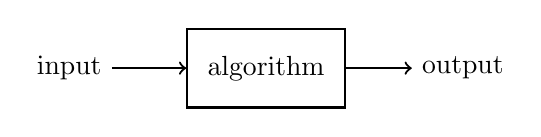
\begin{tikzpicture}[thick]
    \node (input) at (-2.5, 0) {input};
    \node[shape=rectangle,draw=black, minimum width=2cm, minimum height = 1cm] (algorithm) at (0, 0) {algorithm};
    \node (output) at (2.5, 0) {output};

    \draw [->] (input) edge (algorithm);
    \draw [->] (algorithm) edge (output);
  \end{tikzpicture}
\end{figure}

\begin{definition}
  A language \(L\) is a subset of strings \(L \subseteq \Sigma^*\).
\end{definition}

\begin{fact}
  In general, decision problem \(f: \Sigma^* \to \setof{\text{yes}, \text{no}}\) can convert language \(L = \setof{x \in \Sigma^*: f(x) = \text{yes}}\), and conversely, language \(L\) convert to decision problem \(f(x) = \begin{cases} \text{yes}, & x \in L \\ \text{no}, & x \notin L \end{cases}\).
\end{fact}

e.g. \prob{IsPrime}: \(\setof{0, 1}^* \to \setof{\text{yes}, \text{no}}\) is equal to language \(\prob{PRIMES} = \setof{\encoding{x}: x \in \N, \text{\(x\) is prime}} \). \\

Daily programming languages are fun to program, but hard to formalize.

\begin{mdframed}
  Ways to formalize ``algorithm'':
  \begin{enumerate}
    \item Turing Machine ('36)
    \item Lambda Calculus ('36)
    \item Post Machine ('36)
    \item Wang Machine ('50s)
    \item P'' ('64)
  \end{enumerate}
  think they as programming language but ``machines''. Easy to formalize, but annoying to program.
\end{mdframed}

\noindent
{\bf Church-Turing Thesis}: Any real-world algorithm can be simulated by (compiled to) Turing Machines.

\begin{definition}
  {\it ``computable''} means computable by TMs.
\end{definition}

\begin{fact}
  An algo running in time \(T\) in C-like pesudocode can be compiled to a TM running in time \(\approx T^4\).
\end{fact}

\noindent
{\bf Extended Church-Turing Thesis}: Any real-world algorithm can \ldots with at most polynomial slowdown. \\

Our official model: (1-tape, two-way infinite) Turing Machine.

input alphabet \(\Sigma\), tape alphabet \(\Gamma = \Sigma \cup \braces{b}\) where \(b\) is the blank symbol. \ldots many definitions about TM.

\begin{definition}
  The {\it computation trace} of \(M\) on input \(X\) is a sequence of configurations \(C_0, C_1, \ldots, C_n\) where \(C_0\) is the initial configuration, \(C_i\) yields \(C_{i+1}\), and \(C_n\) is an halting configuration.
\end{definition}

\begin{definition}
  TM \(M\) is a {\it decider} if \(M\) on \(X\) halt for all \(X \in \Sigma^*\).
\end{definition}

\begin{definition}
  A TM \(M\) decides language \(L\) iff \(M\) is a decider and \(M\) accept \(X\) iff \(X \in L\), otherwise reject.
\end{definition}

\section{Reading}

\subsection{Sipser 3.1 (Turing Machines)}

\begin{enumerate}
  \item configuration
  \item yield
  \item starting / accepting / rejecting / halting configuration
  \item \(L(M)\): the language of / recognized by \(M\)
  \item decider
  \item Turing recognizable (recursively enumerable language)
  \item Turing decidable (recursive language)
\end{enumerate}

\subsection{Sipser 3.3 (The Definition of Algorithm)}

\begin{enumerate}
  \item hilbert's 10th problem, history background
  \item Church-Turing Thesis
  \item 3-level Description of TM: formal description, impl description, high-level description
\end{enumerate}



\end{document}
